\section{Binning methods}

This section turns from probability models to discretization. We first define binning as a partition of the data domain and briefly review classical rules for choosing the number or width of histogram bins. We then study the three constructions used in the numerical experiments: quantile binning through \texttt{pandas.qcut}, equal-width binning through \texttt{pandas.cut}, and logarithmic binning through geometrically spaced edges. The main analytical result is that, after the essential normalization by bin width, logarithmic binning preserves the exponent of an ideal power-law density while allocating increasingly wide intervals to the sparsely populated tail.

\subsection{What binning is and why there are several strategies}

\begin{definition}[Binning]
Let $I\subseteq\R$ be an interval containing the observed data. A binning of $I$ is a finite ordered partition
\begin{equation}
 I=B_1\cup B_2\cup\cdots\cup B_K,
 \qquad B_j\cap B_k=\varnothing\quad(j\neq k),
\label{eq:partition}
\end{equation}
up to a fixed convention for observations that fall exactly on shared boundaries.
\end{definition}

Equation~\eqref{eq:partition} separates the data domain into mutually exclusive classes whose union recovers the working interval. Membership can be represented compactly by an indicator operator, which is useful both mathematically and computationally.

\begin{definition}[Indicator function]
For a set $A\subseteq\R$, the indicator of $A$ is the function $\mathbf{1}_A:\R\rightarrow\{0,1\}$ defined by
\[
\mathbf{1}_A(x)=
\begin{cases}
1, & x\in A,\\
0, & x\notin A.
\end{cases}
\]
Thus $\mathbf{1}_{B_k}(x_i)$ records whether observation $x_i$ belongs to the $k$th bin.
\end{definition}

For a sample $x_1,\ldots,x_n$, bin occupancy and conservation of the total sample size are then expressed by the paired relations
\begin{subequations}\label{eq:occupancy}
\begin{align}
 n_k &= \sum_{i=1}^{n}\mathbf{1}_{B_k}(x_i),
 \label{eq:occupancy-a}\\
 \sum_{k=1}^{K} n_k &= n.
 \label{eq:occupancy-b}
\end{align}
\end{subequations}
Equation~\eqref{eq:occupancy-a} states that the occupancy $n_k$ is obtained by adding one unit for every observation that belongs to $B_k$ and zero otherwise. Equation~\eqref{eq:occupancy-b} follows from the fact that the bins form a partition: every observation is assigned to exactly one bin, so summing occupancies over all bins recovers the full sample size.

Table~\ref{tab:toy-binning} gives a minimal data set in which the bin name is made explicit. The deliberately skewed values illustrate why the partition geometry matters even before a histogram is drawn.

\begin{table}[htbp]
\centering
\caption{Toy data set assigned to four equal-width bins over the interval $[0,100]$.}
\label{tab:toy-binning}
\begin{tabular}{rrl}
\toprule
Observation & Value $x_i$ & Bin name \\
\midrule
1 & 2.0 & $B_1=[0,25)$ \\
2 & 3.0 & $B_1=[0,25)$ \\
3 & 3.5 & $B_1=[0,25)$ \\
4 & 4.0 & $B_1=[0,25)$ \\
5 & 5.0 & $B_1=[0,25)$ \\
6 & 6.0 & $B_1=[0,25)$ \\
7 & 8.0 & $B_1=[0,25)$ \\
8 & 10.0 & $B_1=[0,25)$ \\
9 & 14.0 & $B_1=[0,25)$ \\
10 & 20.0 & $B_1=[0,25)$ \\
11 & 40.0 & $B_2=[25,50)$ \\
12 & 100.0 & $B_4=[75,100]$ \\
\bottomrule
\end{tabular}
\end{table}

\begin{figure}[!htbp]
\centering
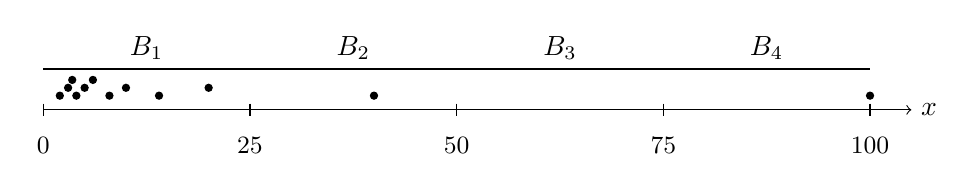
\begin{tikzpicture}[x=0.105cm,y=1cm]
\draw[->] (0,0) -- (105,0) node[right] {$x$};
\foreach \x in {0,25,50,75,100}{\draw (\x,0.08)--(\x,-0.08) node[below=4pt]{\small \x};}
\draw[thick] (0,0.52)--(25,0.52);
\draw[thick] (25,0.52)--(50,0.52);
\draw[thick] (50,0.52)--(75,0.52);
\draw[thick] (75,0.52)--(100,0.52);
\node at (12.5,0.78) {$B_1$};
\node at (37.5,0.78) {$B_2$};
\node at (62.5,0.78) {$B_3$};
\node at (87.5,0.78) {$B_4$};
\foreach \x/\y in {2/0.18,3/0.28,3.5/0.38,4/0.18,5/0.28,6/0.38,8/0.18,10/0.28,14/0.18,20/0.28,40/0.18,100/0.18}{\fill (\x,\y) circle (1.5pt);}
\end{tikzpicture}
\caption{Illustrative equal-width partition of the toy sample in Table~\ref{tab:toy-binning}. Most observations occupy the first interval, the third interval is empty, and the largest observation determines the full linear range.}
\label{fig:toy-binning}
\end{figure}

A histogram supplements the partition with a vertical statistic. For equal-width bins, raw counts or relative frequencies are directly comparable because all intervals have the same width. For unequal-width bins, raw counts confound local probability mass with geometric interval size. A density histogram therefore uses
\begin{equation}
 \widehat f_k=\frac{n_k}{n\,\Delta_k},
 \qquad
 \Delta_k=b_{k+1}-b_k,
\label{eq:density-hist}
\end{equation}
where $b_k$ and $b_{k+1}$ are consecutive bin edges. This normalization guarantees
\begin{equation}
 \sum_{k=1}^{K}\widehat f_k\Delta_k=1.
\end{equation}

There is no universal optimal partition. Sturges \cite{Sturges1926} proposed a classical rule for the number of classes; Scott \cite{Scott1979} derived an asymptotically motivated bandwidth for density estimation; and Freedman and Diaconis \cite{FreedmanDiaconis1981} proposed a robust width proportional to the interquartile range and $n^{-1/3}$. Adaptive strategies also exist. Bayesian Blocks chooses change points by optimizing a statistical fitness function rather than prescribing a constant width \cite{ScargleEtAl2013}, while kernel density estimation replaces hard intervals by smooth local kernels. These methods are useful context, but the present notes focus on three transparent partitions whose geometry can be inspected directly.

The first is equal-width binning: each interval has the same length in the original coordinate. The second is quantile binning: the interval boundaries are empirical quantiles, so occupancies are approximately equal and widths adapt to the local density of observations. The third is logarithmic binning: bin edges are equally spaced after taking logarithms, which means that widths increase geometrically in the original variable. The three choices therefore equalize different objects---width in $x$, probability mass, and width in $\log x$, respectively.

\subsection{Quantile binning with \texttt{pandas.qcut}}

The pandas function \texttt{qcut} implements quantile-based discretization \cite{PandasQcut}. For an integer $K$, it attempts to divide a one-dimensional sample into $K$ groups with equal or nearly equal numbers of observations. Unlike equal-width binning, the geometry is determined by the empirical distribution itself: dense regions receive narrow intervals, while sparse regions receive broad intervals.

\begin{definition}[Empirical quantile]
For observations $x_1,\ldots,x_n$, define the empirical CDF $\widehat F_n$. For $p\in(0,1)$, an empirical quantile can be defined by
\begin{equation}
 \widehat Q_n(p)=\inf\left\{x:\widehat F_n(x)\geq p\right\}.
\end{equation}
A $K$-quantile partition uses the edges
\begin{equation}
 b_k=\widehat Q_n\left(\frac{k}{K}\right),
 \qquad k=0,1,\ldots,K,
\end{equation}
with endpoint conventions chosen to include the sample minimum and maximum.
\end{definition}

The definition makes clear that equal probability content, rather than equal geometric width, is the organizing principle. When the sample is continuous and ties are absent, rank information gives an especially simple occupancy result.

\begin{proposition}[Occupancy of quantile bins]
If the sample has no ties at the chosen quantile boundaries and $K$ divides $n$, an exact rank-based $K$-quantile partition contains $n/K$ observations in every bin.
\end{proposition}

\begin{demonstration}
Order the sample as $x_{(1)}<\cdots<x_{(n)}$. If $K$ divides $n$, define boundaries after the ranks $n/K,2n/K,\ldots,(K-1)n/K$. Each consecutive block then contains exactly $n/K$ order statistics. The absence of ties guarantees that no observation is ambiguous at a shared boundary.
\end{demonstration}

This is the defining practical advantage of \texttt{qcut}: statistical summaries computed inside different bins are based on comparable sample sizes. The method is therefore useful for income deciles, score quintiles, credit-risk bands, or any application in which balanced groups are more important than fixed numerical widths. Its limitation is equally clear: consecutive bins no longer correspond to equal changes in the measured variable, so the physical interpretation of a one-bin displacement varies across the distribution.

For the toy sample used in Sec.~3.1, quartile binning is implemented by
\begin{lstlisting}[caption={Quartile binning with pandas.qcut.}]
import pandas as pd

x = [2, 3, 3.5, 4, 5, 6, 8, 10, 14, 20, 40, 100]
labels, edges = pd.qcut(
    x,
    q=4,
    labels=False,
    retbins=True,
    duplicates="raise",
)
print(edges)
print(labels.to_numpy())
\end{lstlisting}
The corresponding output is
\begin{lstlisting}[caption={Output of the quartile example.},numbers=none]
[  2.      3.875   7.     15.5   100.   ]
[0 0 0 1 1 1 2 2 2 3 3 3]
\end{lstlisting}

Table~\ref{tab:qcut-example} displays the same result as named quartile bins. The widths increase from $1.875$ in the first quartile to $84.5$ in the fourth, while the occupancy remains exactly three observations per bin.

\begin{table}[htbp]
\centering
\caption{Quartile assignment returned by \texttt{qcut} for the toy sample.}
\label{tab:qcut-example}
\begin{tabular}{lll}
\toprule
Values & Bin name & Interval determined by empirical quantiles \\
\midrule
$2,3,3.5$ & $Q_1$ & $[2,3.875]$ \\
$4,5,6$ & $Q_2$ & $(3.875,7]$ \\
$8,10,14$ & $Q_3$ & $(7,15.5]$ \\
$20,40,100$ & $Q_4$ & $(15.5,100]$ \\
\bottomrule
\end{tabular}
\end{table}

In applied data, duplicate quantile edges can arise when many observations share the same value. The pandas implementation allows the user either to raise an error or to remove non-unique edges through the \texttt{duplicates} argument \cite{PandasQcut}. This behavior should be treated as a substantive feature of discrete or rounded data rather than as a purely technical nuisance, because dropping an edge changes the intended number of groups.

\subsection{Equal-width binning with \texttt{pandas.cut}}

The function \texttt{cut} discretizes values according to explicit interval boundaries or, when the number of bins is supplied as an integer, according to equal-width intervals over the observed range \cite{PandasCut}. Its geometry is therefore defined in the original measurement scale. If the working interval is $[a,b]$ and $K$ equal bins are required, the idealized edges are
\begin{equation}
 b_k=a+k\Delta,
 \qquad
 \Delta=\frac{b-a}{K},
 \qquad
 k=0,1,\ldots,K.
\label{eq:cut-edges}
\end{equation}

This construction is natural when additive differences in the original unit are physically meaningful. Age bands of five years, temperature intervals of two degrees, and laboratory measurements reported on a fixed linear scale are typical examples. Equal widths also make raw counts directly comparable because every interval represents the same amount of the underlying variable.

The weakness of the method is its dependence on the total observed range $b-a$. A single extreme observation can enlarge every interval simultaneously, reducing resolution where most observations are concentrated. The toy sample already contains this mechanism: the observation $x=100$ makes a four-bin linear partition much coarser than the quartile partition of the same twelve values.

Using four bins for direct comparison with the \texttt{qcut} example,
\begin{lstlisting}[caption={Equal-width binning with pandas.cut.}]
import pandas as pd

x = [2, 3, 3.5, 4, 5, 6, 8, 10, 14, 20, 40, 100]
labels, edges = pd.cut(
    x,
    bins=4,
    labels=False,
    retbins=True,
    include_lowest=True,
)
print(edges)
print(labels.to_numpy())
\end{lstlisting}
produces
\begin{lstlisting}[caption={Output of the equal-width example.},numbers=none]
[  1.902  26.5    51.     75.5   100.   ]
[0 0 0 0 0 0 0 0 0 0 1 3]
\end{lstlisting}

The first edge is slightly below the observed minimum because pandas extends the range by $0.1\%$ when an integer number of bins is supplied, thereby ensuring that the minimum and maximum are included \cite{PandasCut}. Table~\ref{tab:cut-example} shows the resulting occupancy structure.

\begin{table}[htbp]
\centering
\caption{Equal-width assignment returned by \texttt{cut} for the toy sample.}
\label{tab:cut-example}
\begin{tabular}{lll}
\toprule
Values & Bin name & Interval \\
\midrule
$2,3,3.5,4,5,6,8,10,14,20$ & $B_1$ & $[1.902,26.5]$ \\
$40$ & $B_2$ & $(26.5,51]$ \\
--- & $B_3$ & $(51,75.5]$ \\
$100$ & $B_4$ & $(75.5,100]$ \\
\bottomrule
\end{tabular}
\end{table}

The comparison with Table~\ref{tab:qcut-example} isolates the central distinction. \texttt{qcut} adapts widths to obtain balanced occupancies, whereas \texttt{cut} holds widths approximately fixed and allows occupancies to vary. For broad or heavy-tailed samples the latter variation can be extreme, and Sec.~4 quantifies this effect for the synthetic Pareto experiment.

\subsection{Logarithmic binning}

Logarithmic binning is designed for strictly positive variables whose dynamic range is naturally multiplicative. The method appears prominently in Newman's treatment of power-law data, where ordinary fixed-width histograms become increasingly noisy in the tail because the expected number of observations per bin decreases rapidly \cite{Newman2005}. The same principle has been advocated in other empirical domains, including information science, as a way to aggregate sparse tail observations without discarding the multiplicative structure of the data \cite{Milojevic2010}. More generally, analysis of binned power-law data requires explicit attention to the information lost through aggregation, a point developed statistically by Virkar and Clauset \cite{VirkarClauset2014}.

The construction replaces constant additive increments by constant multiplicative increments. In log coordinates the edges are equally spaced; after transforming back to the original variable, the intervals widen geometrically.

\begin{definition}[Logarithmic binning]
Let $0<x_{\min}<x_{\max}$ and let $K\in\N$. Define
\begin{equation}
 r=\left(\frac{x_{\max}}{x_{\min}}\right)^{1/K}>1.
\end{equation}
The logarithmic bin edges are
\begin{equation}
 b_k=x_{\min}r^k,
 \qquad k=0,1,\ldots,K.
\label{eq:log-edges}
\end{equation}
Equivalently, $\log b_k$ is an arithmetic progression.
\end{definition}

The ratio $r$ controls multiplicative resolution: increasing the bin index by one multiplies the edge by the same factor everywhere in the domain. The width of the $k$th bin is
\begin{equation}
 \Delta_k=b_{k+1}-b_k=(r-1)b_k,
\label{eq:log-width}
\end{equation}
so the absolute width grows linearly with the lower edge. A convenient representative horizontal coordinate is the geometric center
\begin{equation}
 c_k=\sqrt{b_kb_{k+1}}=b_k\sqrt{r},
\end{equation}
which is the midpoint in logarithmic coordinates. This choice respects the same multiplicative geometry that defines the bins.

The widening of the intervals is not an arbitrary smoothing device. In a decreasing heavy-tailed distribution, expected counts per unit linear width become very small at large $x$. Aggregating a wider range in the tail partially compensates for that loss of observations and reduces the visual variance of the empirical histogram. The price is reduced local resolution: binning always discards within-bin information, and excessive logarithmic aggregation can hide curvature, cutoffs, or crossovers. Virkar and Clauset \cite{VirkarClauset2014} quantify this general loss of statistical power for binned power-law data, reinforcing the distinction between a useful visualization and a formal inferential procedure.

A second issue is normalization. Because $\Delta_k$ varies strongly with $k$, raw counts or raw relative frequencies cannot be interpreted as estimates of a common density scale. If the objective is to estimate a PDF, the appropriate histogram height is the width-normalized quantity in Eq.~\eqref{eq:density-hist}. Newman \cite{Newman2005} stresses this correction in logarithmically binned power-law plots, and the following result makes the reason explicit.

\begin{theorem}[Power-law exponent under logarithmic binning]
Suppose $X$ has density $f(x)=Cx^{-\alpha}$ on a range covered by logarithmic bins $[b_k,b_{k+1})$ with $b_{k+1}=rb_k$, where $r>1$ and $\alpha>1$. Then the expected density-histogram height in bin $k$ is proportional to $b_k^{-\alpha}$. Hence the logarithmic-bin density preserves the PDF exponent $\alpha$.
\end{theorem}

\begin{demonstration}
The probability mass of bin $k$ is
\begin{align}
 p_k
 &=\int_{b_k}^{rb_k}Cx^{-\alpha}\,\dd x\\
 &=\frac{C}{\alpha-1}
 \left(b_k^{1-\alpha}-(rb_k)^{1-\alpha}\right)\\
 &=\frac{C}{\alpha-1}
 \left(1-r^{1-\alpha}\right)b_k^{1-\alpha}.
\end{align}
Using Eq.~\eqref{eq:log-width}, the corresponding probability per unit width is
\begin{align}
 \frac{p_k}{\Delta_k}
 &=\frac{C}{(\alpha-1)(r-1)}
 \left(1-r^{1-\alpha}\right)b_k^{-\alpha}.
\end{align}
All factors except $b_k^{-\alpha}$ are constant across bins. Therefore the expected density histogram has the same power-law exponent as the underlying PDF.
\end{demonstration}

The theorem also explains a common plotting error. If logarithmic-bin probabilities $p_k$ are plotted without division by $\Delta_k$, they scale as $b_k^{1-\alpha}$ rather than $b_k^{-\alpha}$, shifting the apparent slope by one. Width normalization is therefore a mathematical requirement for density estimation, not a cosmetic convention. Even after this correction, however, exponent estimation should not be reduced to a straight-line fit on a log--log graph. Maximum-likelihood estimation, explicit treatment of the lower cutoff, goodness-of-fit testing, and comparison with alternative heavy-tailed models remain necessary for empirical inference \cite{ClausetShaliziNewman2009,VirkarClauset2014}.

Figure~\ref{fig:newman-grid} follows the pedagogical logic of Newman \cite{Newman2005} with an independently generated sample of $10^6$ Pareto observations having $\alpha=2.5$. Panel (a) shows the distribution on linear axes, where the tail is visually compressed. Panel (b) uses logarithmic coordinates with fixed linear-width aggregation and exposes the approximate power-law trend, but the far tail becomes noisy because counts become small. Panel (c) uses logarithmically widening bins and width normalization, reducing this heteroscedastic tail noise while preserving the theoretical power-law exponent. Panel (d) shows the empirical CCDF, which avoids histogram boundaries and supplies a complementary view of the same tail.

\begin{figure}[!htbp]
\centering
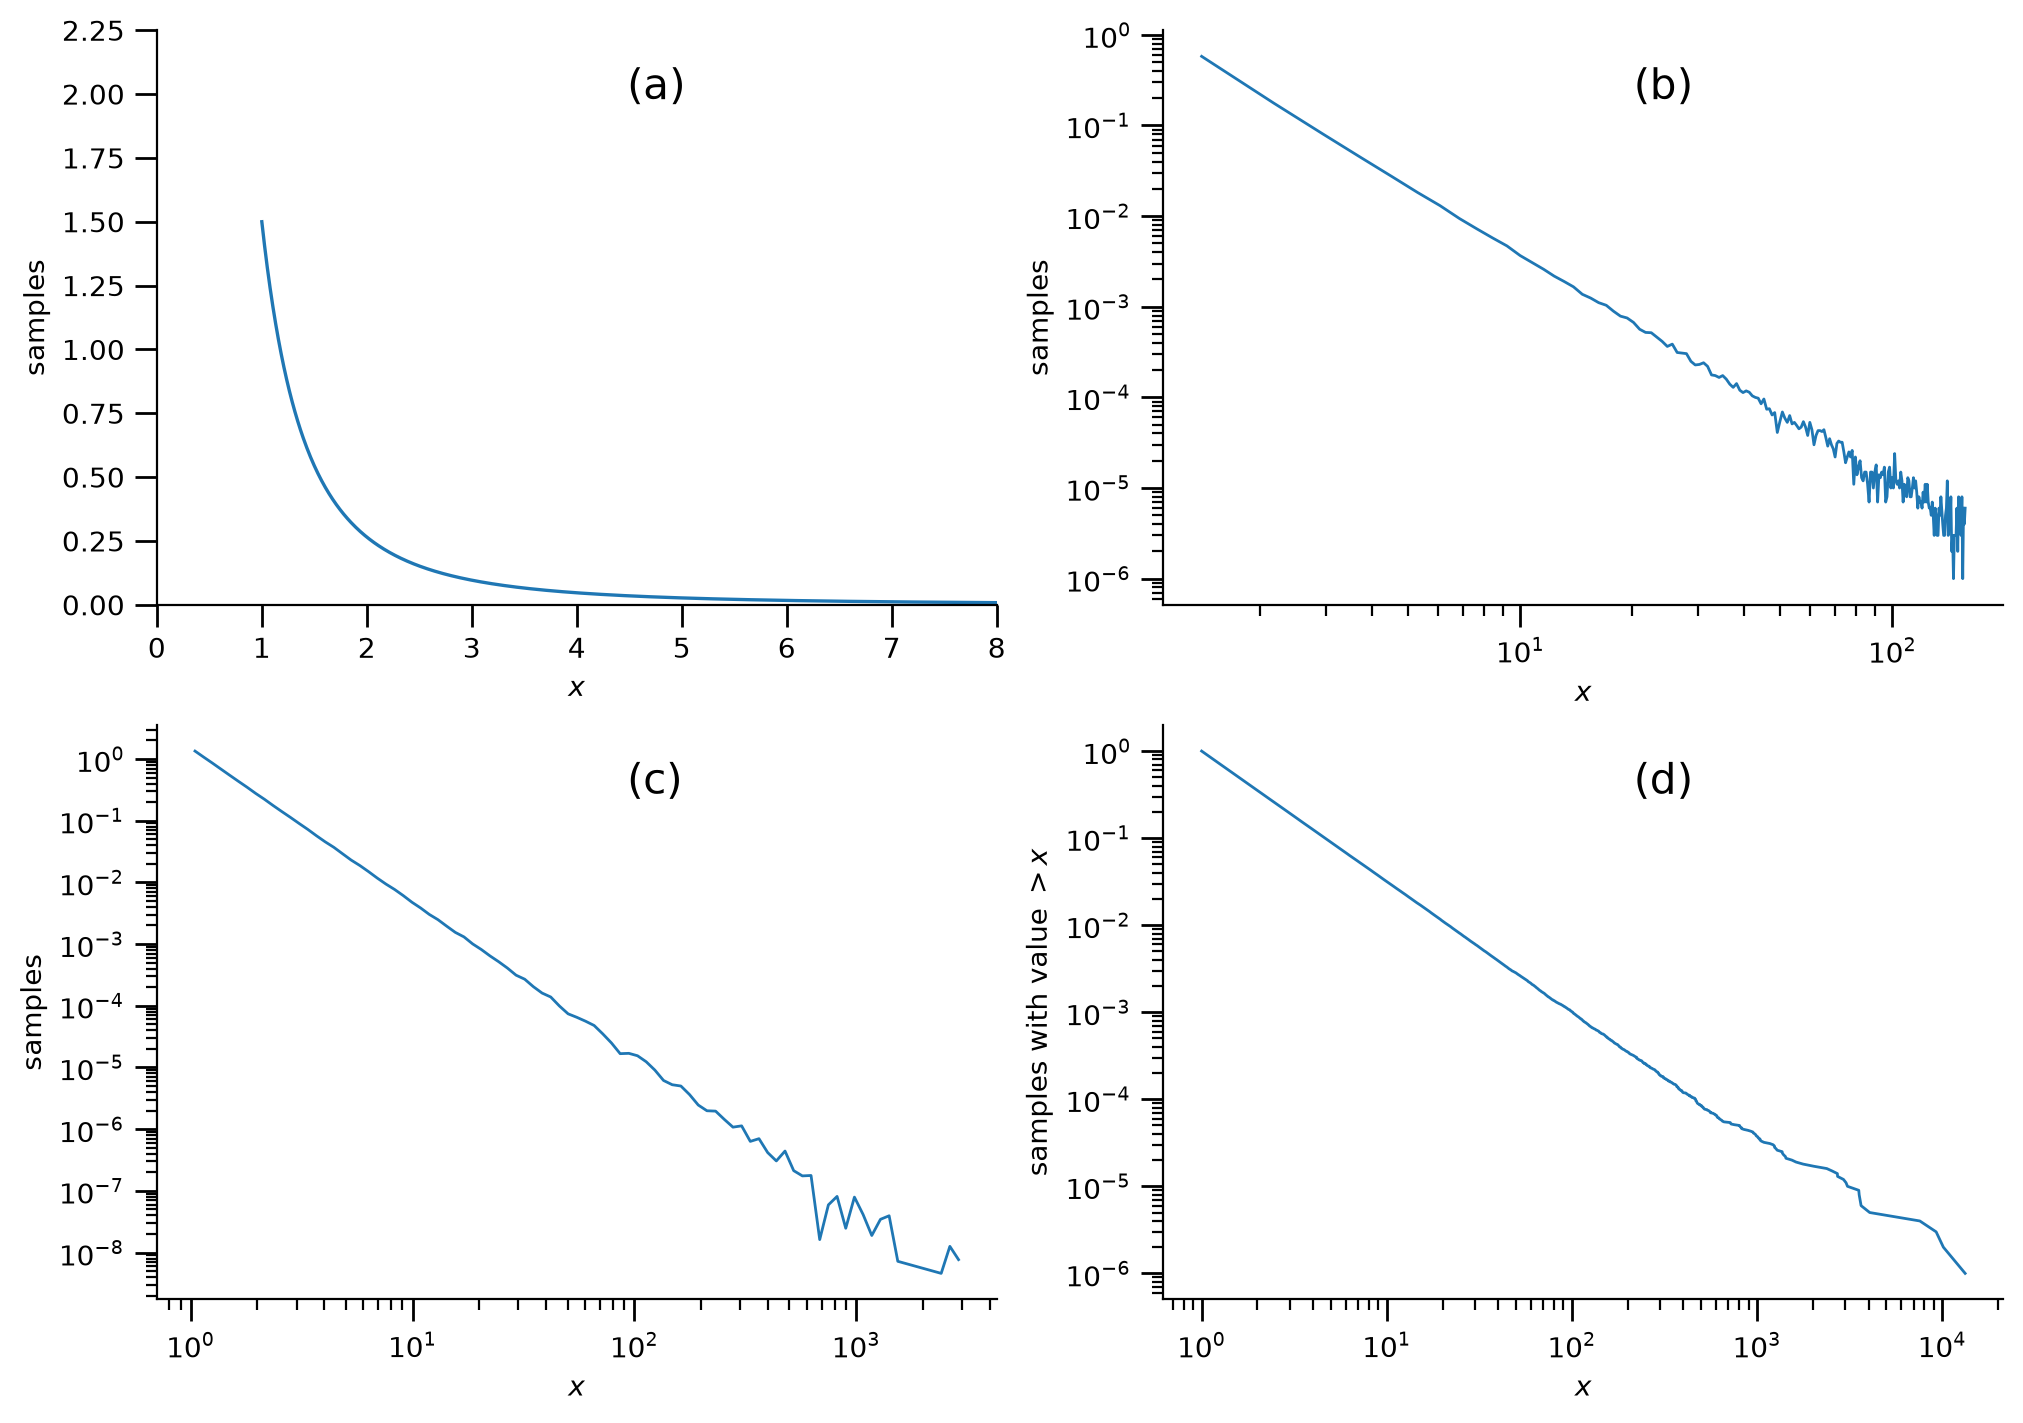
\includegraphics[width=0.72\textwidth]{newman_powerlaw_grid.png}
\caption{Four complementary representations of a synthetic power-law sample, following the pedagogical construction of Newman \cite{Newman2005}: linear representation, log--log representation with fixed linear-width aggregation, logarithmic-bin density, and empirical CCDF.}
\label{fig:newman-grid}
\end{figure}

